%% ----------------------------------------------------------------
%% Authoring.tex
%% ---------------------------------------------------------------- 
\chapter{Authoring Tool} 
\label{Chapter:Authoring Tool}

\begin{preamble}
The authoring tool section details the motivation for creating a tool that is able to produce the \gls{DF} used by the \gls{vgQuestions} plugin. One of the key features was that the tool should be accessible and is able to describe the wide range of features the \gls{vgQuestions} plugin supports.
\end{preamble}

\section{Introduction}
\label{Section:Authoring_Introduction}

An accessible \gls{authoring} was required to allow users to create their own question sets. Within the authoring tool users can create polls and quizzes and overlay them at chosen locations in a video. This avoided the necessity for users of the framework to learn the JavaScript quiz format, thus significantly reducing the technical barrier to entry. 

One key consideration during the implementation of the authoring tool was accessibility. The \gls{WCAG} 2.0 guidelines were kept in mind at all times and adhered to as much as possible.

Care has been taken to ensure that the authoring tool can be easily used within other AngularJS projects, and thorough documentation has been provided to ease this process.

\section{Design} 
\label{Section:Authoring_Design}

\begin{figure}[h]
	\centering
		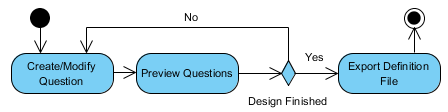
\includegraphics[width=\textwidth]{../figures/authoring_tool/state_diagram.png}

	\caption{
		\label{Figure:Authoring_Tool_state_diagram}
		Image showing a state diagram of how the authoring tool is used.
	}
\end{figure}

Within the authoring tool users have the ability to create questions sets within a video. There could be any number of questions in a set and these could be of many different types. A range of options are given to modify the functionality of each question so as allow the user to create exactly what they need.

At any point the user can preview the quiz they have created on the inbuilt video player. Once they are satisfied with the quiz they can export it for use with videogular-questions externally from the tool.

It was decided to use Bootstrap\footnote{\url{https://github.com/twbs/bootstrap/}} to give a consistent appearance to all of the user interfaces components within the project. This is a HTML, \gls{CSS}, and JavaScript framework for developing webpages.

As an Angular framework is used, any additional functionality is required to be written as directives and controllers. UIBootstrap\footnote{\url{http://angular-ui.github.io/bootstrap/}} provides some Bootstrap components written in \gls{AngularJS}. This provides some of the components required. 

Wireframes were created using this style so that they could easily be directly coded as static HTML to allow a quick demo to be created. 

Two different approaches were suggested for showing the advanced options for the video. A pop up approach hid these from general view to avoid confusing users with lots of options that may be unnecessary. The other approach was to use the accordion structure as we had for the questions. This would be collapsed by default so the options would still be hidden. This was chosen as it was more consistent with the rest of the tool. Wireframes were created to allow for feedback from users and the customer. They can be found in \autoref{Chapter:Authoring Tool Wireframes}.

\section{Implementation}
\label{Section:Authoring_Implementation}
Once the wireframes were drawn up they could be turned into static HTML. Elements of this webpage were then incrementally given the functionality they required. The main challenge was ascertaining how the functionality fitted in with the \gls{AngularJS} Framework. 

Each section of the page had to have its own directive so that independent behaviours could be achieved. This kept the HTML pages short and readable as the behaviour was dealt with by the JavaScript and the styling dealt with by the \gls{CSS}.

Angular allowed the dynamic nature of the data to define the appearance of the page. Sections could be set to appear only when certain attributes were set using ng-switch statements. This meant one section could potentially show many different elements depending on what was selected elsewhere on the page.

\subsection{Data Bubbling}
\label{Section:Authoring_Data_bubbling}

With the authoring tool we have leveraged the ability to use two way binding and watches with AngularJS. This allows us to template a number of reusable elements such as the time picker and means we don't have to rewrite the class each time we wish to use it. This has reduced the time taken to produce the authoring tool.

The root controller holds the global state of the authoring tool. This global state is updated by the child controllers who each own specific parts of the global model. This bubbling of data up the controllers is the key to how the authoring tool has been built.

The preview and generation features utilise this model in the root controller composed from the bubbled models over the child controllers.

\begin{figure}[h]
	\centering
		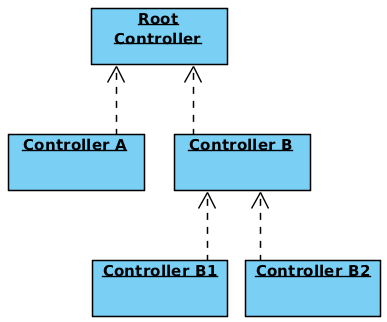
\includegraphics[scale=0.4]{../figures/authoring_tool/controller_bubbling.png} 		
	\caption{\label{Figure: Bubbling model data} Bubbling of model data up controllers} 	
\end{figure}

\autoref{Figure: Bubbling model data} shows the general structure of the controllers and how we have implemented the bubbling up of data. In our implementation we have a large number of controllers and levels to encapsulate the different ways of quiz creation. In this diagram controller A and B will bubble their model data up to the root controller if it changes. If model data in controller B1 or B2 changes, their new model will bubble up to controller B. Controller B will then will then bubble its model combined with the new model data it has received to the root controller.

This bubbling technique works for any number or levels of children provided the model data is correctly bubbled up each layer. It also makes adding new controllers at any point simple as you only need to handle the bubbling of the data up the levels.

Each controller may have one or more children who may or may not hold model data.

\begin{figure}[h]
	\centering
		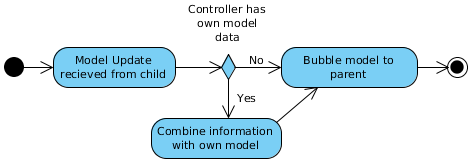
\includegraphics[scale=0.6]{../figures/authoring_tool/bubbling_to_root.png} 		
	\caption{\label{Figure: Bubbling to root} State diagram illustrating decisions when bubbling data to root} 	
\end{figure}

\autoref{Figure: Bubbling to root} demonstrates the decision making process to determine how the controller bubbles the data. Any controller that does not hold important model data will only bubble any information sent to it to the root controller. Any controller that has a model will also bubble its own model and model data received upwards. Therefore the global model is slowly accumulated by bubbling up the data. When it reaches the root controller the global model has been built and is saved for later use.

A controller holding model data stores the state of the controller which is represented by a HTML view. Each view is bound to its specific model using two way data binding. This means when the view is changed by the user the model will be automatically updated.

\begin{figure}[h]
	\centering
		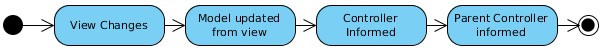
\includegraphics[scale=0.6]{../figures/authoring_tool/two_way_binding.png} 		
	\caption{\label{Figure: Authoring two way binding} Two way binding bubbling method illustrated in an state diagram} 	
\end{figure}

\autoref{Figure: Authoring two way binding} shows the process of the view changing and updating its parent. Each time the model is updated the controller runs any appropriate action to change the display of the view then sends the updated model to its parent. This change is bubbled upwards each level until it reaches the root controller who stores the new data in its global model.

\subsection{Exporting of Data}
\label{Section:Authoring_export_data}

As the user is selecting the options for their quiz, the data will be bubbled up as described in \autoref{Section:Authoring_Data_bubbling}. Once they have finished creating their quiz they will be able to press the export button. When this is pressed the global model is reviewed, and the corresponding \gls{DF} is generated.
\begin{lstlisting}[language=javascript,caption={Base template for authoring tool \gls{DF} generation},label={code:authoringToolTemplate} ]
/* jshint worker: true */
"use strict";

importScripts("WORKER_URL");

/* global loadAnnotations */
loadAnnotations(ANNOTATION_DATA);
\end{lstlisting}

First the global options are processed and the basic file is created. This uses a default template which is stored in the authoring tool. The current template used is shown in \autoref{code:authoringToolTemplate}. This has two sections that are replaced with content that are generated in a later stage. These are `WORKER\_URL' and `ANNOTATION\_DATA'. `WORKER\_URL' is currently replaced by the URL as guessed by the authoring tool. This may need to be modified if the vgQuestions plugin has been modified to move the web worker position. `ANNOTATION\_DATA' is replaced with the generated question data that is generated below.

Once the template has been created, each question set is processed. This involves taking all the settings for the question set, storing it the question set format, and then processing and generating JavaScript for each question in the question set.

When generating the JavaScript for each question the question type is used to generate a set of attributes specific to that question type. The attributes generated are as defined in the class diagram \autoref{Figure:questions_class_diagram} and these are added to the question.

For some questions, there will be a number of different annotation questions added to the question set. One example is when the quiz author has selected that a user may return to a specific point if they fail a question. This will add a question asking the user if they wish to review the section of the video containing the answer to the question. This template is shown in \autoref{code:authoringToolTemplateRewatchSection} and has the variables `QUESTION\_ID' and `TIME' which will be replaced with the data from the question the user has enabled the option on.

Once an individual question has been generated the next question in the question set will be processed.

Once all of the questions in a question set has been processed it will continue onto the next question set.

Some options allow you to add results at the end of the video. These settings are stored up and once the all question sets have been processed this is added onto the end of the `ANNOTATION\_DATA' string.

\begin{lstlisting}[language=javascript,caption={The final \gls{DF} is offered for downloading using a data blob URL},label={code:authoringToolFileDownload} ]
var url = "data:text/json;charset=utf8," + encodeURIComponent(data);
window.open(url, "_blank");
window.focus();
\end{lstlisting}

Once all of these options have been calculated the final template is produced. The template string have their content inserted to generate the finished \gls{DF}. To allow the user to download the file easily we construct a blob url with the code in \autoref{code:authoringToolFileDownload}. Without using a data URL we would require the user to copy the text generated and save it. As this was not a user friendly option so we investigated possible other uses. Offering a file for download was problematic because JavaScript does not have any write permission for files since it is client side. The data blob URL solution provides an acceptable solution by mocking up file URL with data. This may encounter issues with larger files due to the max length permitted in a URL but we have not yet seen these issues occur.

\subsection{Preview tool}

The preview tool works similar to the export tool (\autoref{Section:Authoring_export_data}) by generating the \gls{DF} and creating the blob URL. Once this has been done this is passed to the vgQuestion plugin embedded in the authoring tool which loads up the newly created quiz.

This allows for immediate feedback when creating the quiz and makes it easier to create a quiz for non technical users (\cref{Req:User friendliness}). Since we have embedded the vgQuestions plugin we will be sure that this will react the same when added to a website using the plugin.

\section{Conclusions}
\label{Section:Authoring_Conclusion}

The tool we have produced allows a user to create the \gls{DF} in the correct format that can be used vgQuestions to display user created quizzes.

\cref{Req:Keyboard accessibility} outlines the importance of accessibility so we have designed the authoring tool to be as accessible as possible. \autoref{Section: Conformance of Authoring Tool} details our conformance to the \gls{WCAG} standards. In \autoref{Section:Testing_Authoring_tool_accessibility} we have ran through a number of testing methods applied to the authoring tool to demonstrate that it is accessible and outlined any further issues.

\autoref{Figure:Authoring_Tool} is an image showing our final user interface. The colour scheme was chosen to be high contrasting to fulfil \cref{Req:Use of colour}. In addition the CSS used to set this colour scheme is in a single place and is easy to change as to a users requirement.

To further decrease the barrier to entry (\cref{Req:User friendliness}) we used the \gls{Videogular} and \gls{vgQuestions} plugin to allow a preview of the quiz they have created. One of the useful side effects of \cref{Req:Standalone} has meant that it has been easy to integrate \gls{vgQuestions} into the authoring tool.

There may be some more work needed to investigate how large a JavaScript quiz file may be produced when using the data blob URL approach to allow the user to download the file. While no limits problems have occurred during testing this is something that will need to be kept in mind. \todo{What is this trying to say?}

\begin{landscape}

\begin{figure}[h]
	\centering
		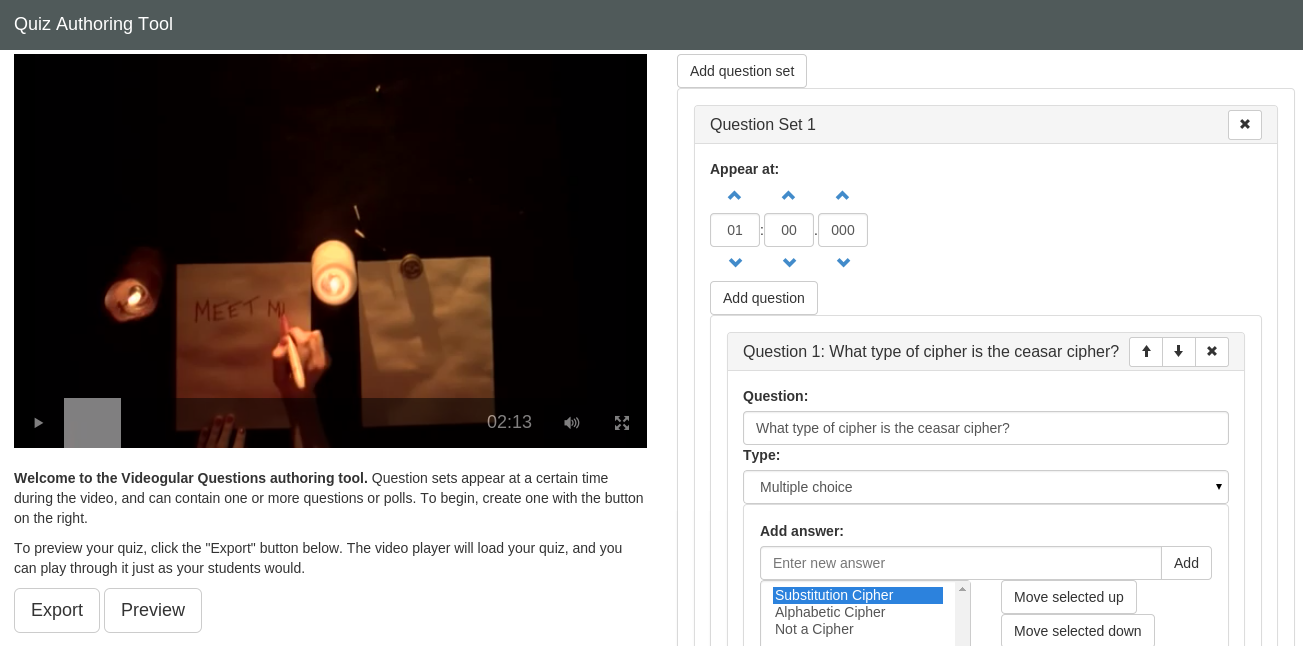
\includegraphics[width=0.8\paperheight]{../figures/authoring_tool_example.png}

	\caption{
		\label{Figure:Authoring_Tool}
		Image showing the final authoring tool being used
	}
\end{figure}

\end{landscape}
